\documentclass[a4paper,12pt]{article}
\usepackage[utf8]{inputenc}
\usepackage[T1]{fontenc}
\usepackage{hyperref}
\usepackage{geometry}
\usepackage{booktabs}
\usepackage{array}
\usepackage{longtable}
\usepackage{multirow}
\usepackage{pgfplots}
\usepackage{tikz}
\usepackage{tabularx}

\geometry{a4paper, margin=2.5cm}
\pgfplotsset{compat=1.18}

\hypersetup{
    colorlinks=true,
    linkcolor=red,
    urlcolor=cyan,
    citecolor=blue
}

\begin{document}

% ── Titolo ────────────────────────────────────────────────────────
\begin{center}
{\LARGE\textbf{Milestone 4 Report}\\[0.4em]
\Large TrentoParking}\\[1em]
{\large Team 12}\\[0.3em]
{\large 4 Giugno 2026}
\end{center}

\vspace{1.5em}
\tableofcontents
\newpage

% ── 1. Sezione Introduttiva ───────────────────────────────────────
\section{Sezione Introduttiva}

\subsection{Team Members}

\begin{table}[h!]
\centering
\begin{tabular}{|l|c|l|}
\hline
\textbf{Nome e Cognome} & \textbf{Matricola} & \textbf{Account Github} \\
\hline
David Dorobantu  & 234467 & \url{https://github.com/DavidDorobantu} \\
Riccardo Gonzato & 246476 & \url{https://github.com/Gonzo04} \\
Matteo Sepa      & 243283 & \url{https://github.com/sepamatteo} \\
\hline
\end{tabular}
\caption{Membri del team}
\end{table}

\subsection{Project Idea}

TrentoParking è un'applicazione web dedicata al noleggio di posti auto privati.
L'obiettivo del progetto è permettere ai proprietari di parcheggi privati di mettere
a disposizione il proprio posto auto quando non utilizzato, mentre gli utenti possono
cercare e prenotare rapidamente un parcheggio disponibile tramite una mappa interattiva.
L'applicazione vuole ridurre il tempo necessario alla ricerca di parcheggio, migliorare
la mobilità urbana e ottimizzare l'utilizzo degli spazi privati inutilizzati.

\subsection{Links}

\begin{itemize}
  \item Repository Github: \url{https://github.com/Gonzo04/TrentoParking}
  \item Link Apiary: \url{https://trentoparking.docs.apiary.io/#}
  \item Deploy: l'applicazione è eseguita in locale. Per avviarla: clonare il
        repository, configurare le variabili d'ambiente seguendo
        \texttt{.env.example}, eseguire \texttt{npm install} nelle
        cartelle \texttt{backend/} e \texttt{frontend/}, quindi avviare con
        \texttt{npm run dev} in entrambe. L'app sarà disponibile su
        \texttt{http://localhost:5173}.
  \item Account demo:
  \begin{itemize}
    \item \textbf{Admin}  --- email: \texttt{admin@trentoparking.it}, password: \texttt{admin123}
    \item \textbf{Host}   --- email: \texttt{host@trentoparking.it}, password: \texttt{host123}
    \item \textbf{Utente} --- email: \texttt{mario.rossi@gmail.com}, password: \texttt{password123}
  \end{itemize}
\end{itemize}

% ── 2. Sezione Generale ───────────────────────────────────────────
\section{Sezione Generale}

\subsection{Strategia di Branching}

Il team ha mantenuto la strategia di branching basata sul modello \textit{GitFlow
semplificato senza develop} adottata nel primo sprint.
I branch utilizzati sono:

\begin{itemize}
  \item \textbf{main}: contiene esclusivamente versioni stabili e funzionanti
        dell'applicazione.
  \item \textbf{feature/*}: branch dedicati allo sviluppo di specifiche funzionalità.
\end{itemize}

Rispetto al primo sprint, nel secondo sprint il team ha lavorato in parallelo su un
numero maggiore di branch contemporaneamente, integrando le modifiche tramite Pull
Request su GitHub prima di ogni merge in \texttt{main}.
I principali branch del secondo sprint sono stati:

\begin{itemize}
  \item \texttt{feature/spot-photos} --- caricamento foto per i posti privati
  \item \texttt{feature/chat} --- sistema di messaggistica tra utente e host
  \item \texttt{feature/review} --- sistema di recensioni dei posti privati
  \item \texttt{feature/admin-dashboard} --- pannello di amministrazione
  \item \texttt{feature/booking-safe-spot-status} --- protezione eliminazione posti con
        prenotazioni future attive
  \item \texttt{refactor/frontend-structure} --- riorganizzazione della struttura del
        frontend in \texttt{pages/}, \texttt{features/} e \texttt{components/common/}
\end{itemize}

Il flusso di lavoro ha previsto: sviluppo su branch dedicato $\rightarrow$ apertura
Pull Request $\rightarrow$ revisione del codice $\rightarrow$ merge in \texttt{main}.
Questa procedura ha permesso di rilevare e risolvere i conflitti in modo controllato,
in particolare in occasione del refactoring del frontend.

\subsection{Product Backlog}

Di seguito il Product Backlog aggiornato con le user story introdotte nel secondo
sprint (ID 13--17).

\begin{longtable}{|c|l|p{4.5cm}|c|p{3cm}|}
\hline
\textbf{ID} & \textbf{Name} & \textbf{User story} & \textbf{Imp.} & \textbf{How to Demo} \\
\hline
\endfirsthead
\hline
\textbf{ID} & \textbf{Name} & \textbf{User story} & \textbf{Imp.} & \textbf{How to Demo} \\
\hline
\endhead
1  & Registrazione         & Come utente voglio registrarmi tramite email e password.                                    & 100 & Account creato e email di verifica ricevuta. \\
\hline
2  & Verifica Email        & Come utente voglio verificare il mio account tramite email.                                & 60  & Click sul link: account attivato. \\
\hline
3  & Login                 & Come utente voglio effettuare il login per accedere alla piattaforma.                      & 100 & Credenziali corrette: redirect alla home. \\
\hline
4  & Password reset        & Come utente voglio recuperare la password dimenticata.                                     & 60  & Email di reset ricevuta, password aggiornata. \\
\hline
5  & Mappa interattiva     & Come utente voglio visualizzare una mappa per trovare parcheggi.                           & 60  & Mappa centrata su Trento con marker parcheggi. \\
\hline
6  & Visualizzazione parcheggio & Come utente voglio vedere i posti disponibili sulla mappa.                            & 80  & Marker caricati dinamicamente dal backend. \\
\hline
7  & Filtro per raggio     & Come utente voglio filtrare i parcheggi per distanza.                                      & 30  & Slider raggio: mappa filtra i posti. \\
\hline
8  & Menu parcheggi card   & Come utente voglio vedere i parcheggi in una lista laterale.                               & 80  & Sidebar sincronizzata con la mappa. \\
\hline
9  & Selezione dalla mappa & Come utente voglio selezionare un parcheggio dalla mappa o dalla lista.                    & 50  & Selezione marker: dettagli del posto. \\
\hline
10 & Prenotazione          & Come utente voglio prenotare un posto auto disponibile.                                    & 100 & Prenotazione confermata con pagamento mock. \\
\hline
11 & Recensioni            & Come utente voglio lasciare recensioni ai proprietari dei parcheggi.                       & 60  & Recensione inserita dopo prenotazione conclusa. \\
\hline
12 & Messaggi              & Come utente voglio comunicare con il proprietario del parcheggio.                          & 70  & Chat aperta: messaggi inviati e ricevuti. \\
\hline
13 & Foto posti            & Come host voglio caricare foto del mio posto per renderlo più attrattivo.                  & 30  & Foto caricate dall'host visibili nel dettaglio posto. \\
\hline
14 & Gestione posti host   & Come host voglio gestire i miei posti (pubblicazione, modifica, eliminazione).             & 60  & Host modifica ed elimina i propri posti dalla dashboard. \\
\hline
15 & Prenotazioni ricevute & Come host voglio visualizzare le prenotazioni ricevute sui miei posti.                     & 50  & Host accede alla sezione e vede dettagli e stato. \\
\hline
16 & Profilo utente        & Come utente voglio modificare i miei dati personali.                                       & 40  & Utente aggiorna nome e targa dalla pagina profilo. \\
\hline
17 & Pannello admin        & Come amministratore voglio gestire utenti, posti e prenotazioni.                           & 40  & Admin modifica ruoli e annulla prenotazioni dal pannello. \\
\hline
\caption{Product Backlog aggiornato}
\end{longtable}

\subsection{Definizione di Done}

Una funzionalità viene considerata \textit{Done} quando soddisfa tutti i seguenti
criteri (invariata rispetto allo Sprint 1):

\begin{itemize}
  \item il codice è stato implementato e caricato su Github;
  \item il codice compila senza errori;
  \item sono stati eseguiti test manuali e/o automatici;
  \item il codice è stato revisionato da almeno un altro membro del team;
  \item non sono presenti bug critici noti;
  \item la user story associata soddisfa i requisiti definiti durante lo sprint planning.
\end{itemize}

% ── 3. Sprint 2 ───────────────────────────────────────────────────
\section{Sprint 2}

\subsection{Goal}

L'obiettivo principale dello Sprint 2 è stato completare le funzionalità core
dell'applicazione, trasformando TrentoParking da un prototipo di autenticazione
e visualizzazione mappa in un sistema di prenotazione parcheggi completo e
multi-ruolo.\\[0.4em]
Durante questo sprint il team si è concentrato su:

\begin{itemize}
  \item completamento e consolidamento del sistema di prenotazione con pagamento;
  \item implementazione del sistema di recensioni per i posti prenotati;
  \item caricamento e visualizzazione di foto per i posti privati;
  \item sistema di chat tra utente e host;
  \item gestione del profilo utente;
  \item dashboard host per la gestione dei propri posti e delle prenotazioni ricevute;
  \item pannello di amministrazione per la gestione di utenti, posti e prenotazioni;
  \item refactoring della struttura frontend per migliorare la manutenibilità.
\end{itemize}

\subsection{Sprint Planning}

Durante lo Sprint Planning il team ha analizzato le user story prioritarie e
stimato il carico di lavoro.

\begin{longtable}{|c|>{\small}p{3.5cm}|p{4cm}|c|c|}
\hline
 & \textbf{User Story} & \textbf{Task} & \textbf{Volunt.} & \textbf{Est.} \\
\hline
\endfirsthead
\hline
 & \textbf{User Story} & \textbf{Task} & \textbf{Volunt.} & \textbf{Est.} \\
\hline
\endhead
\multirow{17}{*}{\rotatebox{90}{Sprint \#2}}
 & \multirow{6}{3.5cm}{Come utente voglio prenotare un posto auto disponibile e gestire le mie prenotazioni.}
 & Completamento API prenotazioni & Matteo & 3 \\
\cline{3-5}
 & & UI calendario e form prenotazione & Matteo & 4 \\
\cline{3-5}
 & & Sistema pagamento (mock) & Matteo & 3 \\
\cline{3-5}
 & & Lista e cancellazione prenotazioni & Matteo & 3 \\
\cline{3-5}
 & & Testing prenotazioni & Matteo & 2 \\
\cline{3-5}
 & & Deploy servizio prenotazioni & Matteo & 1 \\
\cline{2-5}
 & \multirow{3}{3.5cm}{Come host voglio caricare foto del mio posto.}
 & API upload foto (Multer) & Matteo & 3 \\
\cline{3-5}
 & & Integrazione upload frontend & Matteo & 3 \\
\cline{3-5}
 & & Visualizzazione foto nel dettaglio & Matteo & 2 \\
\cline{2-5}
 & \multirow{4}{3.5cm}{Come utente voglio lasciare recensioni ai proprietari.}
 & Modello e API recensioni & David & 3 \\
\cline{3-5}
 & & UI modale recensione e stelle & David & 3 \\
\cline{3-5}
 & & Calcolo e visualizzazione media & David & 3 \\
\cline{3-5}
 & & Testing recensioni & David & 2 \\
\cline{2-5}
 & \multirow{4}{3.5cm}{\small Come utente voglio comunicare con il proprietario del parcheggio.}
 & Modello e API messaggi & Matteo & 3 \\
\cline{3-5}
 & & UI ChatModal con polling & Matteo & 4 \\
\cline{3-5}
 & & Integrazione chat nelle prenotazioni & Matteo & 2 \\
\cline{3-5}
 & & & & \\
\cline{2-5}
 & \multirow{3}{3.5cm}{Come utente voglio modificare i miei dati personali.}
 & API modifica profilo & Riccardo & 2 \\
\cline{3-5}
 & & UI pagina profilo & David & 4 \\
\cline{3-5}
 & & & & \\
\cline{2-5}
 & \multirow{3}{3.5cm}{Come host voglio gestire i miei posti auto.}
 & API CRUD posti host & Riccardo & 4 \\
\cline{3-5}
 & & UI dashboard gestione posti & Riccardo & 4 \\
\cline{3-5}
 & & Blocco eliminazione posti con prenotazioni & Riccardo & 2 \\
\cline{2-5}
 & \multirow{3}{3.5cm}{\small Come host voglio visualizzare le prenotazioni ricevute.}
 & API prenotazioni ricevute & Riccardo & 3 \\
\cline{3-5}
 & & UI lista prenotazioni ricevute & Riccardo & 3 \\
\cline{3-5}
 & & & & \\
\cline{2-5}
 & \multirow{4}{3.5cm}{\small Come amministratore voglio gestire utenti, posti e prenotazioni.}
 & Backend API admin e middleware & Matteo & 5 \\
\cline{3-5}
 & & UI AdminDashboard (3 tab) & Matteo & 5 \\
\cline{3-5}
 & & Integrazione e testing admin & Matteo & 2 \\
\cline{3-5}
 & & & & \\
\cline{2-5}
 & \multirow{3}{3.5cm}{Refactoring e miglioramenti tecnici.}
 & Refactoring struttura frontend & Riccardo & 5 \\
\cline{3-5}
 & & Miglioramenti UI e stile & David & 4 \\
\cline{3-5}
 & & Bug fix generali & David & 4 \\
\hline
\multicolumn{4}{|r|}{\textbf{Total}} & \textbf{90} \\
\hline
\caption{Sprint Backlog Sprint 2}
\end{longtable}

\subsubsection{Burndown Chart}

Il Burndown Chart mostra l'andamento dello sprint e il completamento progressivo
delle attività (totale: 90 story point, durata: 21 giorni). L'asse Y indica i
punti rimanenti; l'asse X i giorni trascorsi dall'inizio dello sprint.

\begin{figure}[h!]
\centering
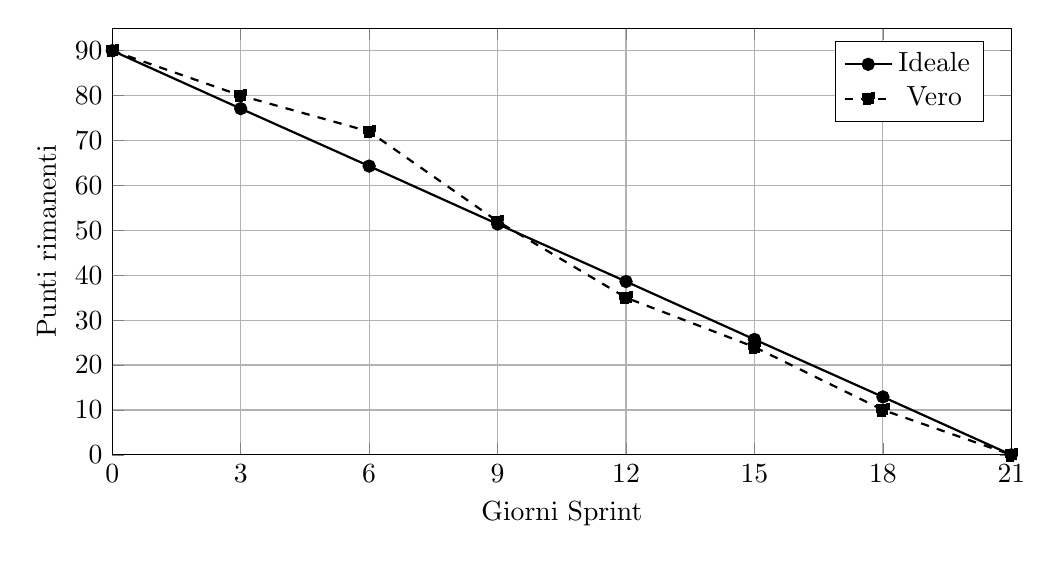
\begin{tikzpicture}
\begin{axis}[
  width=13cm, height=7cm,
  xlabel={Giorni Sprint},
  ylabel={Punti rimanenti},
  xmin=0, xmax=21,
  ymin=0, ymax=95,
  xtick={0,3,6,9,12,15,18,21},
  ytick={0,10,20,30,40,50,60,70,80,90},
  legend pos=north east,
  grid=both,
  grid style={line width=0.2pt, draw=gray!30},
  major grid style={line width=0.4pt, draw=gray!60},
]
\addplot[mark=*, thick] coordinates {
  (0,90) (3,77.1) (6,64.3) (9,51.4) (12,38.6) (15,25.7) (18,12.9) (21,0)
};
\addlegendentry{Ideale}
\addplot[mark=square*, thick, dashed] coordinates {
  (0,90) (3,80) (6,72) (9,52) (12,35) (15,24) (18,10) (21,0)
};
\addlegendentry{Vero}
\end{axis}
\end{tikzpicture}
\caption{Burndown Chart Sprint 2}
\end{figure}

\subsection{Test Cases}

Di seguito sono riportati 20 test case relativi alle funzionalità implementate
nello Sprint 2.

\begin{longtable}{|l|c|p{2.8cm}|p{2.5cm}|p{1.8cm}|p{2.8cm}|}
\hline
\textbf{User Story} & \textbf{ID} & \textbf{Description} & \textbf{Test Case Data} & \textbf{Precond.} & \textbf{Expected Result} \\
\hline
\endfirsthead
\hline
\textbf{User Story} & \textbf{ID} & \textbf{Description} & \textbf{Test Case Data} & \textbf{Precond.} & \textbf{Expected Result} \\
\hline
\endhead
\multirow{5}{*}{Prenotazione}
 & 01 & Prenotazione riuscita        & Slot libero, targa: AA000BB    & Loggato          & Prenotazione creata, stato \texttt{\small IN\_ATT\_PAG}. \\
\cline{2-6}
 & 02 & Slot già occupato            & Slot già prenotato             & Loggato          & Errore disponibilità. \\
\cline{2-6}
 & 03 & Pagamento prenotazione       & Click ``Paga ora''             & \texttt{\small IN\_ATT}  & Stato diventa PAGATA. \\
\cline{2-6}
 & 04 & Cancellazione prenotazione   & Click ``Annulla''              & Prenotazione attiva & Stato diventa ANNULLATA. \\
\cline{2-6}
 & 05 & Lista prenotazioni utente    & Accesso a ``Le mie prenotazioni'' & Loggato       & Lista prenotazioni mostrata. \\
\hline
\multirow{3}{*}{Foto posti}
 & 06 & Upload foto valide           & 3 file JPG                     & Host loggato     & Foto salvate e visibili nel dettaglio. \\
\cline{2-6}
 & 07 & Upload più di 10 foto        & 11 file selezionati            & Host loggato     & Errore: limite 10 foto. \\
\cline{2-6}
 & 08 & Visualizzazione foto         & Apertura dettaglio posto       & Foto caricate    & Carosello immagini visibile. \\
\hline
\multirow{4}{*}{Recensioni}
 & 09 & Inserimento recensione valida & 4 stelle, commento testuale   & Prenotazione conclusa & Recensione salvata, media aggiornata. \\
\cline{2-6}
 & 10 & Recensione duplicata         & Seconda recensione stessa prenotazione & Recensione già presente & Errore duplicato. \\
\cline{2-6}
 & 11 & Visualizzazione media stelle & Accesso scheda posto           & $\geq$1 recensione & Media e totale recensioni mostrati. \\
\cline{2-6}
 & 12 & Recensioni per host          & Accesso pagina recensioni host & Recensioni in DB & Lista con stelle e commento. \\
\hline
\multirow{3}{*}{Chat}
 & 13 & Invio messaggio              & Testo: ``Posso parcheggiare alle 15?'' & Prenotazione attiva & Messaggio inviato e visibile. \\
\cline{2-6}
 & 14 & Ricezione messaggi           & Messaggio inviato dall'altro utente & Chat aperta  & Messaggio appare entro 4 secondi. \\
\cline{2-6}
 & 15 & Accesso non autorizzato      & Utente terzo chiama GET /chat/:id & Non coinvolto & Errore 403. \\
\hline
\multirow{3}{*}{Gestione posti host}
 & 16 & Pubblicazione nuovo posto    & Nome, indirizzo, tariffa oraria & Host loggato   & Posto creato e visibile sulla mappa. \\
\cline{2-6}
 & 17 & Modifica posto               & Modifica tariffa oraria        & Posto esistente  & Tariffa aggiornata. \\
\cline{2-6}
 & 18 & Eliminazione con prenotazioni & Click ``Elimina''             & Prenotazioni future attive & Errore: eliminazione bloccata. \\
\hline
\multirow{2}{*}{Pannello admin}
 & 19 & Cambio ruolo utente          & Ruolo: UTENTE $\rightarrow$ HOST & Admin loggato  & Ruolo aggiornato in DB. \\
\cline{2-6}
 & 20 & Annullamento da admin        & Click ``Annulla'' su prenotazione & Admin loggato & Stato diventa ANNULLATA. \\
\hline
\caption{Test Cases Sprint 2}
\end{longtable}

\subsection{Sprint Review}

Durante la Sprint Review il team ha effettuato una dimostrazione delle funzionalità
implementate nel secondo sprint.\\[0.3em]
Sono state presentate:

\begin{itemize}
  \item il flusso completo di prenotazione di un posto auto (ricerca, selezione,
        prenotazione e pagamento mock);
  \item il caricamento e la visualizzazione di foto associate ai posti privati;
  \item il sistema di recensioni con calcolo della media stelle per host e per posto;
  \item la chat tra utente prenotante e host con aggiornamento automatico;
  \item la dashboard host per la gestione dei posti pubblicati e la visualizzazione
        delle prenotazioni ricevute;
  \item la pagina di modifica del profilo utente;
  \item il pannello di amministrazione con gestione di utenti, posti e prenotazioni.
\end{itemize}

La discussione successiva si è concentrata su:

\begin{itemize}
  \item miglioramenti all'esperienza utente nel flusso di prenotazione;
  \item possibili ottimizzazioni delle performance lato frontend;
  \item gestione dei casi limite nella chat (messaggi lunghi, connessioni lente).
\end{itemize}

\subsection{Product Backlog Refinement}

Durante il refinement il team ha rianalizzato il Product Backlog alla luce del
lavoro svolto nel secondo sprint. Tutte le user story pianificate per Sprint 2
(ID 10--17) sono state completate e marchiate come \textit{Done}: il sistema di
prenotazione, le foto dei posti, le recensioni, la chat, la gestione del profilo,
la dashboard host e il pannello admin sono stati consegnati e verificati secondo
la Definizione di Done adottata dal team.\\[0.3em]
Il team ha inoltre rivalutato le priorità residue: poiché tutte le 17 user story
del Product Backlog risultano completate, non sono state aggiunte nuove voci né
modificate le stime esistenti. La discussione si è concentrata sulla qualità del
prodotto finale, identificando come possibili aree di miglioramento futuro
l'ottimizzazione delle performance del frontend e l'introduzione di notifiche
in tempo reale per la chat in sostituzione del polling attuale.

\subsection{Sprint Retrospective}

Durante la retrospective il team ha analizzato gli aspetti positivi e negativi
dello sprint.

\subsubsection{Aspetti positivi}

\begin{itemize}
  \item ottima collaborazione tramite Pull Request e revisione del codice;
  \item parallelismo efficace nello sviluppo grazie a branch separati;
  \item buona coerenza visiva dell'interfaccia mantenuta tra le diverse funzionalità;
  \item completamento di tutte le user story pianificate per lo sprint;
  \item risoluzione efficace dei conflitti di merge anche in presenza di modifiche
        sovrapposte (refactoring frontend durante sviluppo attivo).
\end{itemize}

\subsubsection{Criticità riscontrate}

\begin{itemize}
  \item il refactoring della struttura frontend a metà sprint ha introdotto conflitti
        che hanno richiesto tempo aggiuntivo per la risoluzione;
  \item alcuni bug (visualizzazione foto mancanti, bug nel pagamento) sono stati
        scoperti solo dopo il merge in \texttt{main}, evidenziando la necessità di
        test più sistematici prima del merge;
  \item la stima delle ore per il pannello admin si è rivelata ottimistica a causa
        della complessità dell'interfaccia a tre tab.
\end{itemize}

\subsubsection{Pratiche Agile adottate}

Il team ha adottato le seguenti pratiche Agile durante lo sprint:

\begin{itemize}
  \item \textbf{Sprint Planning}: all'inizio dello sprint il team ha definito
        collettivamente le user story da sviluppare, stimato i task e assegnato
        i volontari per ciascuna attività.
  \item \textbf{Sprint Review}: al termine dello sprint il team ha effettuato
        una demo delle funzionalità implementate, raccogliendo feedback.
  \item \textbf{Sprint Retrospective}: il team ha analizzato il processo di lavoro
        per identificare punti di forza e aree di miglioramento.
  \item \textbf{Feature branching e Pull Request}: ogni funzionalità è stata
        sviluppata su un branch dedicato e integrata tramite Pull Request con
        revisione del codice, in linea con il principio di continuous integration.
\end{itemize}

\subsubsection{Design Thinking}

Il team ha applicato alcuni principi del Design Thinking durante lo sviluppo:

\begin{itemize}
  \item \textbf{Empathize}: le funzionalità sono state progettate tenendo conto
        delle esigenze dei diversi ruoli (utente, host, amministratore), con
        interfacce dedicate per ciascuno.
  \item \textbf{Prototype}: le schermate principali sono state prototipate
        iterativamente, con aggiustamenti UI basati sull'utilizzo reale durante
        i test manuali.
  \item \textbf{Test}: ogni funzionalità è stata testata manualmente prima del
        merge, con test case documentati nella sezione dedicata.
\end{itemize}

\subsubsection{Dinamiche di gruppo}

Il team ha mantenuto una collaborazione efficace per tutta la durata dello sprint:

\begin{itemize}
  \item la comunicazione è avvenuta in modo costante tramite messaggistica
        istantanea e incontri periodici di allineamento;
  \item la suddivisione dei task è stata bilanciata, con ciascun membro
        responsabile di aree funzionali distinte;
  \item la revisione reciproca del codice tramite Pull Request ha favorito
        la condivisione delle conoscenze tecniche all'interno del team.
\end{itemize}

% ── 4. Sezione Finale ────────────────────────────────────────────
\section{Sezione Finale}

\subsection{Diagramma del Deploy}

\begin{figure}[h!]
\centering
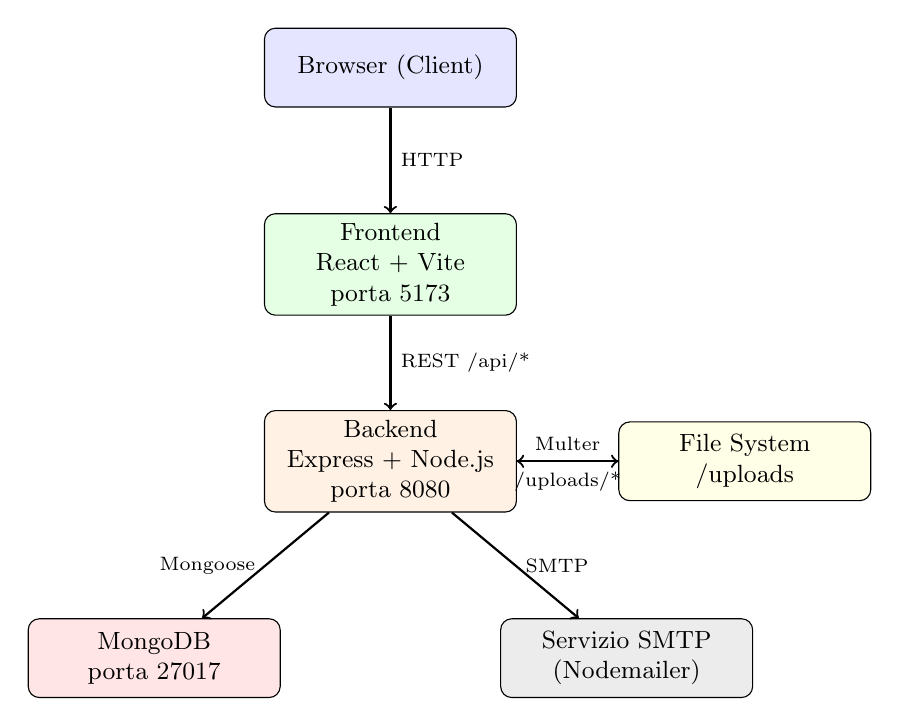
\begin{tikzpicture}[
  box/.style={rectangle, draw, rounded corners, minimum width=3.2cm,
    minimum height=1cm, align=center, font=\small},
  ext/.style={box, fill=gray!15},
  arr/.style={->, thick}
]
\node[box, fill=blue!10]   (browser)  at (4,9)   {Browser (Client)};
\node[box, fill=green!10]  (frontend) at (4,6.5) {Frontend\\React + Vite\\porta 5173};
\node[box, fill=orange!10] (backend)  at (4,4)   {Backend\\Express + Node.js\\porta 8080};
\node[box, fill=red!10]    (mongo)    at (1,1.5) {MongoDB\\porta 27017};
\node[ext]                 (smtp)     at (7,1.5) {Servizio SMTP\\(Nodemailer)};
\node[box, fill=yellow!10] (fs)       at (8.5,4) {File System\\/uploads};

\draw[arr] (browser)  -- node[right, font=\scriptsize]{HTTP} (frontend);
\draw[arr] (frontend) -- node[right, font=\scriptsize]{REST /api/*} (backend);
\draw[arr] (backend)  -- node[left,  font=\scriptsize]{Mongoose} (mongo);
\draw[arr] (backend)  -- node[right, font=\scriptsize]{SMTP} (smtp);
\draw[arr] (backend)  -- node[above, font=\scriptsize]{Multer} (fs);
\draw[arr, dashed] (fs) -- node[below, font=\scriptsize]{/uploads/*} (backend);
\end{tikzpicture}
\caption{Architettura di deploy di TrentoParking}
\end{figure}

L'applicazione è composta da tre livelli principali:

\begin{itemize}
  \item \textbf{Frontend}: applicazione React servita da Vite (porta 5173). Comunica
        con il backend esclusivamente tramite chiamate REST autenticate con JWT.
  \item \textbf{Backend}: server Express (porta 8080) che espone le API REST, gestisce
        l'autenticazione JWT, il caricamento file tramite Multer e l'invio email
        tramite Nodemailer.
  \item \textbf{Database}: istanza MongoDB (porta 27017) con Mongoose come ODM. I file
        caricati vengono salvati nella cartella \texttt{backend/uploads/} e serviti
        come file statici.
\end{itemize}

\subsection{Stack Tecnologico}

\subsubsection*{Backend}

\begin{table}[h!]
\centering
\begin{tabular}{|l|l|l|}
\hline
\textbf{Libreria / Framework} & \textbf{Versione} & \textbf{Utilizzo} \\
\hline
Node.js      & runtime & Runtime JavaScript server-side \\
Express      & 4.21.0  & Framework HTTP e routing REST \\
Mongoose     & 8.7.0   & ODM per MongoDB \\
MongoDB      & 7.x     & Database NoSQL documentale \\
bcryptjs     & 2.4.3   & Hashing delle password \\
jsonwebtoken & 9.0.2   & Autenticazione stateless JWT \\
Multer       & 2.1.1   & Upload file multipart (foto posti) \\
Nodemailer   & 8.0.7   & Invio email (verifica account, reset password) \\
dotenv       & 16.4.5  & Gestione variabili d'ambiente \\
cors         & 2.8.6   & Cross-Origin Resource Sharing \\
\hline
\end{tabular}
\caption{Stack tecnologico backend}
\end{table}

\subsubsection*{Frontend}

\begin{table}[h!]
\centering
\begin{tabular}{|l|l|l|}
\hline
\textbf{Libreria / Framework} & \textbf{Versione} & \textbf{Utilizzo} \\
\hline
React         & 19.2.4 & Libreria UI dichiarativa \\
React DOM     & 19.2.4 & Rendering React nel browser \\
Vite          & 8.0.1  & Build tool e dev server \\
Leaflet       & 1.9.4  & Mappa interattiva \\
React-Leaflet & 5.0.0  & Binding React per Leaflet \\
lucide-react  & 1.14.0 & Libreria icone SVG \\
\hline
\end{tabular}
\caption{Stack tecnologico frontend}
\end{table}

\subsection{Conclusioni}

Il secondo sprint ha permesso di trasformare TrentoParking da un prototipo di
autenticazione e visualizzazione mappa in un'applicazione web completa per il
noleggio di posti auto privati.

Le funzionalità principali --- prenotazione con pagamento mock, caricamento foto,
recensioni, chat utente-host, gestione posti da parte dell'host e pannello di
amministrazione --- sono state implementate e integrate con successo. La struttura
del codice è stata riorganizzata in \texttt{pages/}, \texttt{features/} e
\texttt{components/common/} per favorire la manutenibilità.

Il team ha dimostrato una buona capacità di lavorare in parallelo su branch
separati e di integrare le modifiche tramite Pull Request, gestendo anche situazioni
di conflitto complesse come quelle introdotte dal refactoring del frontend. Le
criticità emerse --- in particolare la gestione dei merge e la stima delle ore per
funzionalità ad alta complessità di interfaccia --- hanno fornito spunti concreti
per migliorare il processo di sviluppo.

\end{document}
